\documentclass[12pt]{report}
\usepackage[numbers]{natbib}
\usepackage[french]{babel}  % Définit la langue du document
\usepackage[utf8]{inputenc}  % Encodage UTF-8 pour les accents
\usepackage[T1]{fontenc}
\usepackage[a4paper, top=2.5cm, bottom=2.5cm, left=2cm, right=2cm]{geometry}
\usepackage{graphicx}
\usepackage{titlesec}
\usepackage{subcaption}
\usepackage{url}
\usepackage{algorithm}
\usepackage{algpseudocode}
\usepackage{listings}   
\usepackage{tcolorbox}
\usepackage{float}
\usepackage[colorlinks=true, linkcolor=blue, citecolor=blue, urlcolor=blue]{hyperref}
\usepackage{csquotes}

\titleformat{\chapter}[hang] % Use hang style (title below number)
  {\normalfont\LARGE\bfseries} % Formatting of the title
  {\thechapter.} % Number format (just 1., 2., etc.)
  {1em} % Space between number and title
  {} % Code before the title

\lstdefinestyle{sharpc}{language=[Sharp]C, rulecolor=\color{blue!80!black}}

\bibliographystyle{plain}

\begin{document}

% Page de garde
\begin{titlepage}
    \begin{center}
        \vspace*{3.25cm}  

        % Logos
       
\includegraphics[width=0.5\textwidth]{images/logos/inria_logo.png} \\[1cm]

        \rule{\linewidth}{0.5mm} \\[0.5cm]
        {\huge \textbf{Documentation haut-niveau du prototype Dora}} \\[0.5cm]
        \rule{\linewidth}{0.5mm} \\[2cm]

        \textit{Auteurs:} \\ 
        \textbf{Aymen ALI YAHIA, Mohammed DOUIDY } \\[3cm]

        \textbf{\today}
        

        \vfill  % Ensures remaining space is pushed to the bottom
    \end{center}
\end{titlepage}

% Table des matières sur la deuxième page
\newpage
\tableofcontents
\newpage

\chapter{Introduction}
\section{Prototype Dora}
Ce prototype a pour but de simplifier la mise en place d’expériences permettant l’exploration de la perception d'un utilisateur à l'aide plusieurs modifications dans la scène, hors du champ de vision ainsi qu'à l’intérieur.
Le prototype est un prefab, portable sur n'importe quelle scène \texttt{Unity} créée avec la pipeline \texttt{URP}. Le prefab est situé dans le répertoire \texttt{Assets/Prefabs/tracking} nommé \texttt{Tracking System}.
Ce dernier est constitué de deux parties, une partie pour les gestionnaires et une autre pour les éléments de visualisation.
\begin{figure}[H]
    \centering
    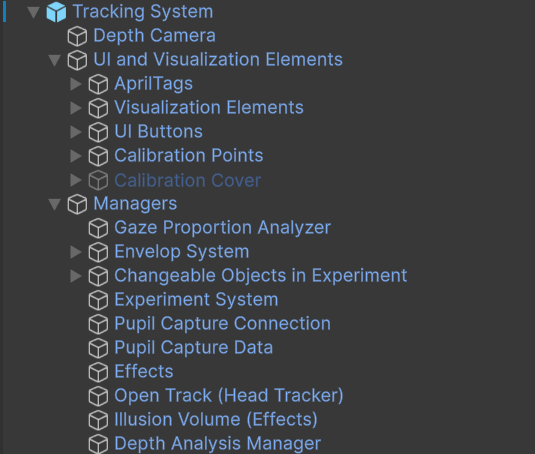
\includegraphics[width=0.5\linewidth]{images/prefab.png}
    \caption{Illustration du prefab \texttt{Unity}}
    \label{fig:prefab}
\end{figure}

Pour les gestionnaires, chaque GameObject est associé à un ou plusieurs scripts, qui nous permettent de paramétrer les différents gestionnaires afin de modifier les expériences comme voulu.
Pour les éléments de visualisations, ils sont hiérarchisés de façon à séparer le interface utilisateur et les autres éléments de visualisations, qui peuvent être modifiés.
\section{Setup matériel}
La configuration optimale est de connecter les différents trackers sur une même machine, cette dernière va envoyer les données des trackers à la machine qui exécute la scène \texttt{Unity}.
Cette configuration permet d'alléger la charge sur le CPU de la machine qui exécute la scène \texttt{Unity}, permettant d'avoir le moins de latence possible.
\begin{figure}[H]
    \centering
    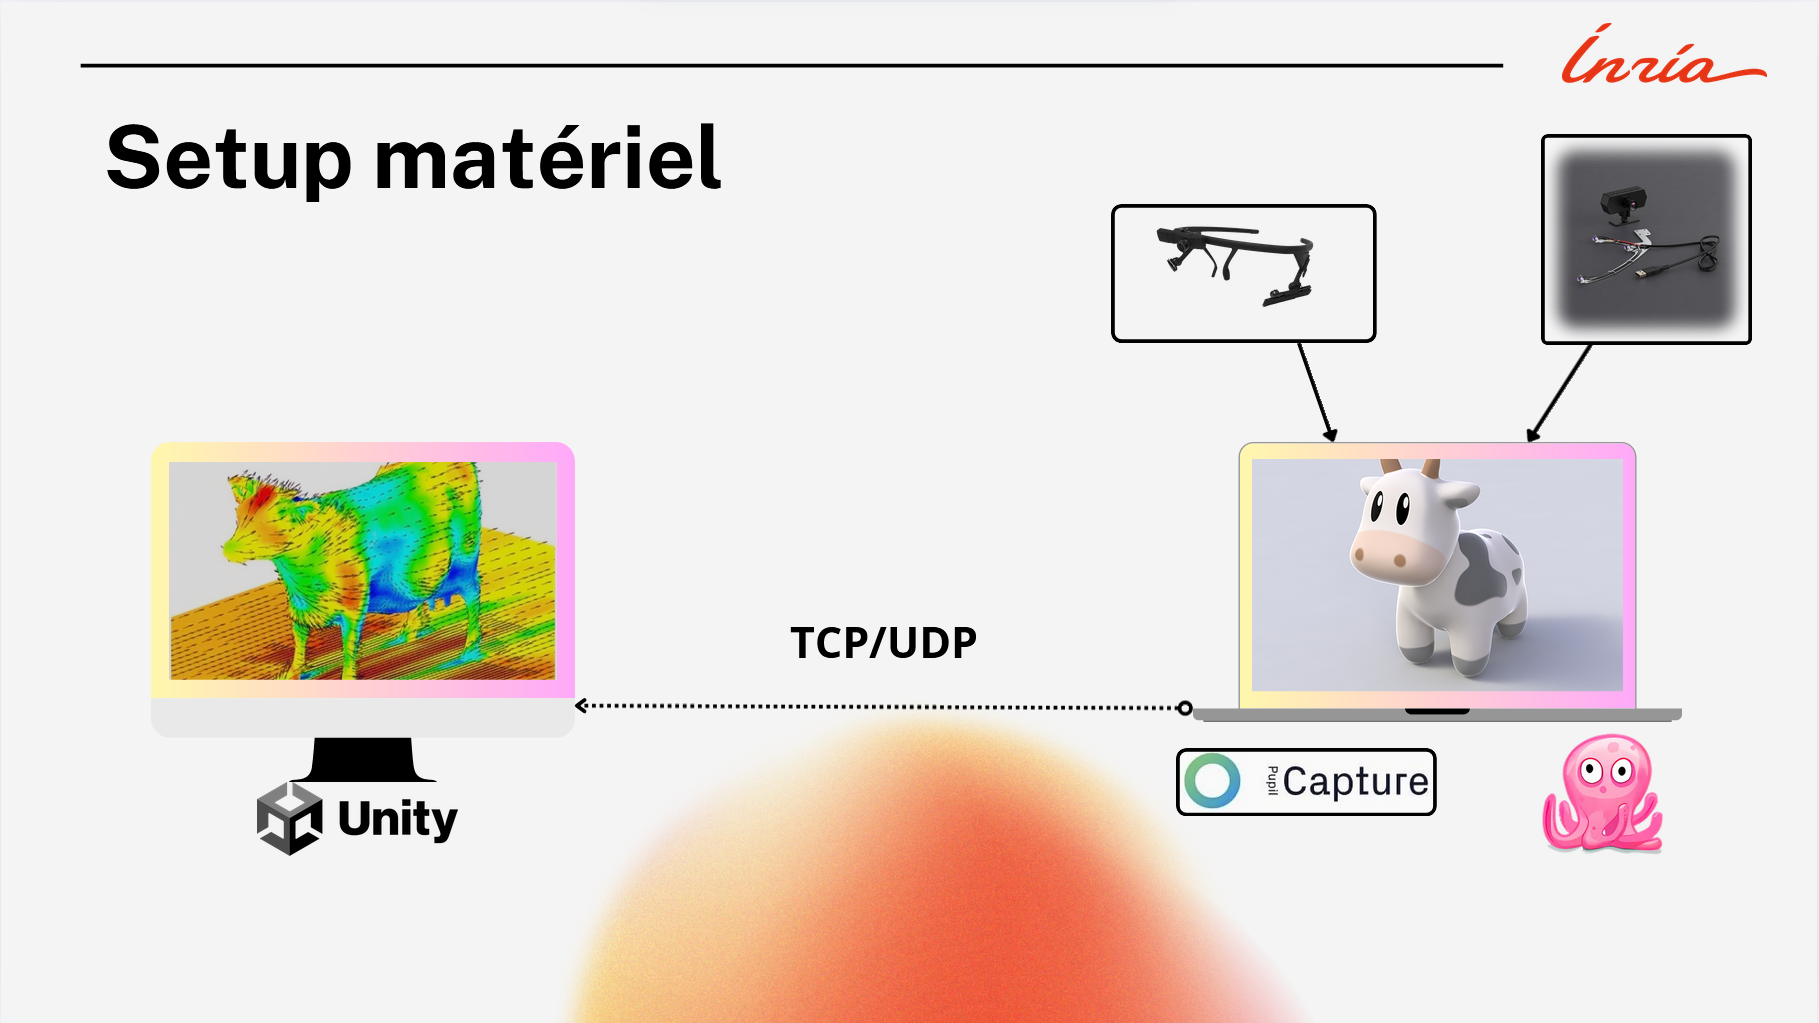
\includegraphics[width=0.7\linewidth]{images/setup_matériel.png}
    \caption{Illustration du setup matériel}
    \label{fig:setup_matériel}
\end{figure}
Cependant, il est possible de lancer tous les programmes sur une même machine, à condition que le CPU soit assez performant et que la machine ait environ 24 GB de RAM.

\chapter{Eye-tracking}
\section{Présentation générale}
Le système de eye-tracking permet à l'utilisateur modifier dynamiquement la scène 3D en bougeant le regard. Il utilise deux cameras infrarouge et une camera monde avec des marqueurs placés sur la scène \texttt{Unity}afin d'avoir la position du regard dans la scène en temps réel. La position parmi, d'autres informations, est envoyée via le réseau. Ces informations permettent de réaliser un certain nombre de calculs permettant d'obtenir les objects contenus dans la zone de regard, des informations de profondeurs, etc...
\section{Installation et paramètrage de Pupil Capture}
Sachant qu'une version modifiée de Pupil Capture est nécessaire pour faire fonctionner ce prototype, voici les étapes à suivre afin de compiler et d'exécuter le programme:
\begin{itemize}
    \vspace{2mm}
    \item Installer et télécharger \texttt{Python 3.11}.
    \item Lancer \texttt{Powershell} en admin au niveau du répertoire \texttt{Dora/pupil}.
    \item Créer un environnement virtuel avec \texttt{Python 3.11} via la commande: 
    \begin{lstlisting}[language=bash]
    python -3.11 -m venv venv
    \end{lstlisting}
    \item Lancez l’environnement virtuel via la commande :
    \begin{lstlisting}[language=bash]
    .\venv\Scripts\activate
    \end{lstlisting}
    \item Installer les dépendances via les commande:
    \begin{lstlisting}[language=bash]
    python -m pip install --upgrade pip setuptools
    python -m pip install -r requirements.txt
    \end{lstlisting}
    \item Lancer le programme dans le répertoire \texttt{pupil\textunderscore src} via la commande :
    \begin{lstlisting}[language=bash]
    .\pupil\pupil_src\main.py capture
    \end{lstlisting}
    \item Si jamais la version de \texttt{NumPy} pose problème, effectuer les commandes suivantes:
    \begin{lstlisting}[language=bash]
    pip uninstall numpy
    pip install "numpy<2.0"
    \end{lstlisting}

\end{itemize}
Certains paramètres de Pupil Capture influent sur les performances (latence et justesse) du eye-tracker. Voici quelques paramètres à modifier pour avoir de meilleures performances:
\begin{figure}[H]
    \centering
    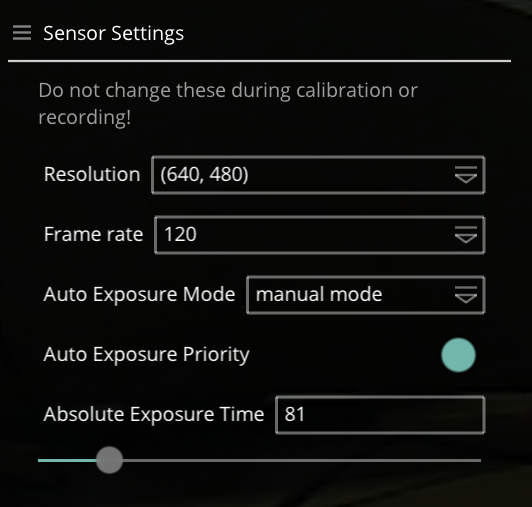
\includegraphics[width=0.4\linewidth]{images/world_settings.png}
    \caption{Paramètres à utiliser pour la camera monde}
    \label{fig:world_settings}
\end{figure}
Pour la camera monde, les paramètres les plus importants sont la résolution et l'exposition.
On trouve que la résolution 640x480 est le bon compromis entre détection stable des tags et faible latence. Pour améliorer la détection des tags et aussi la latence, on diminue le \texttt{Absolute Exposure Time} autant que possible (en ayant \texttt{manual mode} sélectionné dans le champ \texttt{Auto Exposure Mode}). On vérifie la stabilité de détection des tags à la stabilité de la surface détecté autour des tags.

\begin{figure}[H]
    \centering
    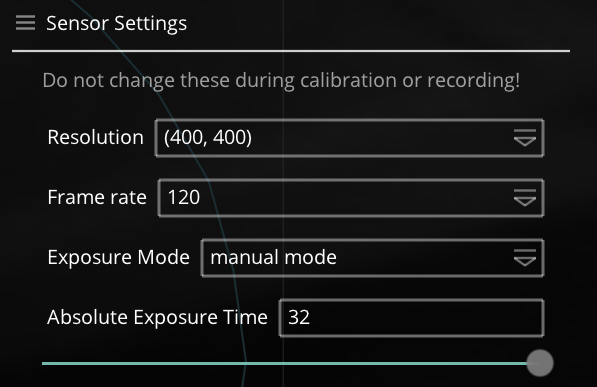
\includegraphics[width=0.5\linewidth]{images/eye_settings.png}
    \caption{Paramètres à utiliser pour les cameras des yeux}
    \label{fig:eye_settings}
\end{figure}
Pour les cameras des yeux, le paramètre principal est l'exposition. Il faut diminuer ce dernier (en ayant \texttt{manual mode} sélectionné dans le champ \texttt{Exposure Mode}) pour avoir une détection stable des pupilles et une bonne latence. La résolution n'impacte que très peu la détection des pupilles, on choisit donc la plus haute résolution disponible.

\section{Bonnes pratiques}

Pour garantir une bonne qualité de suivi oculaire, il est recommandé d’utiliser la pipeline 3D lorsqu’une robustesse face aux mouvements est requise, et la pipeline 2D lorsque la priorité est la justesse de la détection. Il faut aussi de désactiver tous les plugins non utilisés pour limiter les interférences et améliorer la stabilité du système.

Avant toute calibration, plusieurs réglages sont nécessaires pour assurer une détection optimale. Il est essentiel de bien centrer l’œil à l’aide des molettes et des extensions du capteur, d’ajuster le ROI (à activer dans chaque fenêtre de retour des caméras infrarouges) ainsi que la zone de détection de la pupille, en faisant des tours avec les yeux, afin qu’elles soient aussi réduites que possible tout en englobant l’ensemble des mouvements de l’œil. La taille des tags utilisés dans la scène doit également être adaptée pour garantir une détection stable, dépendant la taille de l'écran utilisé pendant les expériences. Le focus de la caméra monde doit être précisément ajusté afin d’optimiser la détection des tags, et l’exposition doit être réglée manuellement : pour la caméra monde, pour stabiliser la détection des tags, et pour les caméras oculaires, afin d’atteindre une confiance proche de 1.
\begin{figure}[H]
    \centering
    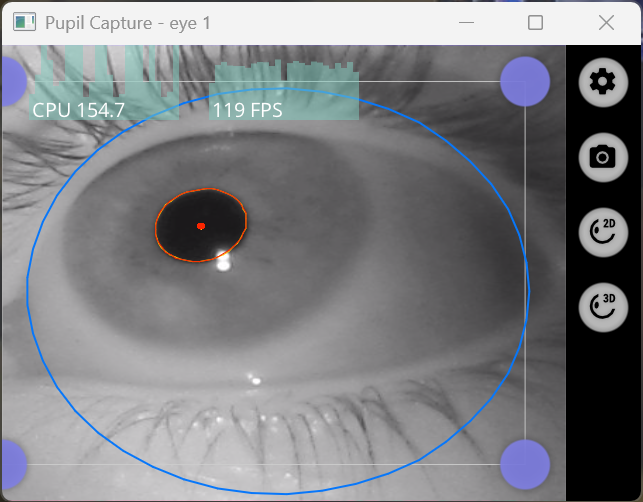
\includegraphics[width=0.5\linewidth]{images/roi_eye.png}
    \caption{Illustration de la zone d’intérêt (rectangle en bleu) et la zone de mouvement de l’œil (ellipse en bleu)}
    \label{fig:placeholder}
\end{figure}

Certaines conditions physiologiques peuvent influencer la qualité de la détection. Il est conseillé d’éviter le maquillage, en particulier le mascara, ainsi que des cils trop fournis, car ceux-ci perturbent la détection des pupilles. De plus, les yeux de couleur claire sont généralement moins bien perçus par les algorithmes, ce qui peut affecter la fiabilité des mesures.

La phase de calibration est très importante, étant le facteur de variabilité le plus impactant. Il est recommandé d’utiliser une calibration à 9 points pour de meilleurs résultats. Durant cette phase, l’utilisateur doit rester aussi neutre et stable que possible pour assurer une correspondance fiable entre les points de calibration et les données recueillies.
La calibration peut se faire sur chacune des deux machines, aucune différence n'a été remarqué, à condition que la distance entre l'utilisateur et la machine de calibration soit similaire à la distance entre l'utilisateur et la machine pour les expériences.

Enfin, pendant toute la durée de l’expérience, il est crucial d’éviter les mouvements brusques qui peuvent altérer significativement la précision du suivi oculaire à cause des mouvements du eye-tracker sur le visage. Si la justesse du regard n’est pas satisfaisante, il ne faut pas hésiter à relancer plusieurs calibrations dans le logiciel Capture jusqu’à obtenir un résultat optimal, qui est autour des 1 dégrée.

Pour plus d'information sur les bonnes pratiques, \href{https://docs.pupil-labs.com/core/best-practices/}{les recommendations du constructeur}
\newpage
\section{Pupil Capture dans {Unity}}

\subsection{Architecture générale du système}
\subsubsection{Connexion de Pupil Capture dans \texttt{Unity}}
Pour lancer la scène avec le eye-tracking, il faut remplir le champ \texttt{Pupil Capture Connection} avec l'adresse IP situé dans l'onglet connexion de Pupil Capture. Choisir la bonne addresse par rapport au mode de connexion utilisé.

\begin{figure}[H]
    \centering
    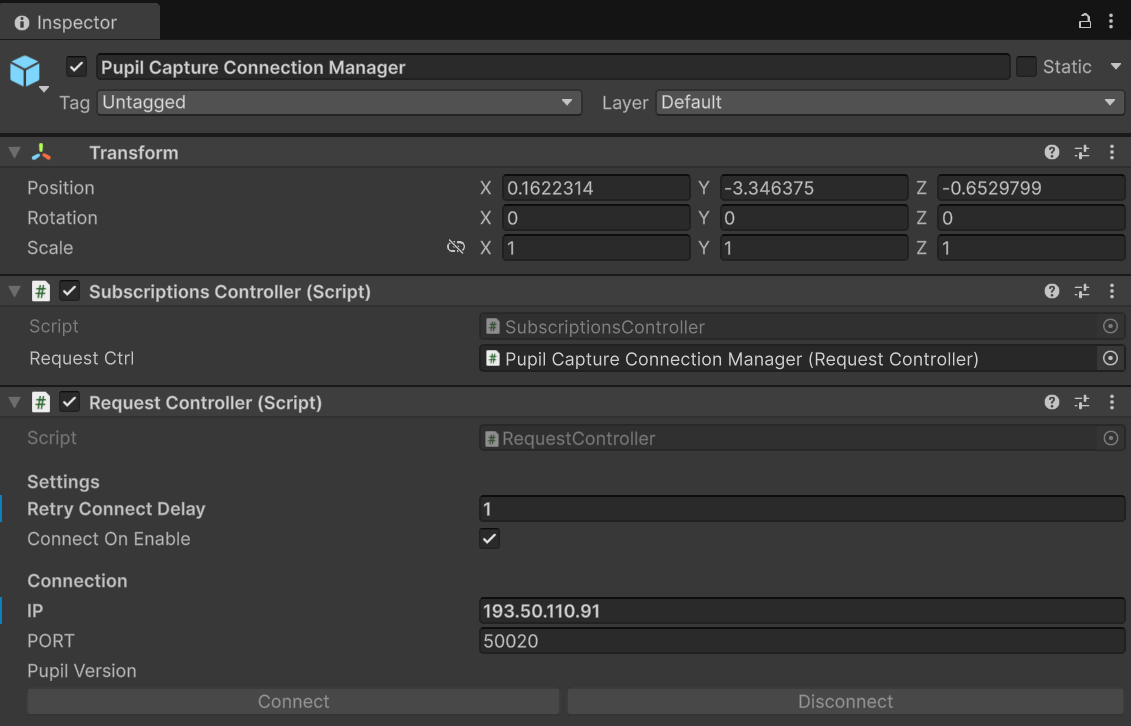
\includegraphics[width=0.5\linewidth]{images/connection_scene.png}
    \caption{Connexion de Pupil Capture avec \texttt{Unity}}
    \label{fig:connection_scene}
\end{figure}
\subsubsection{Configuration de Pupil Capture Data}
Ensuite, il faut remplir tous les champs de \texttt{Pupil Capture Data} (Gaze Manager) comme suit:
\begin{figure}[H]
    \centering
    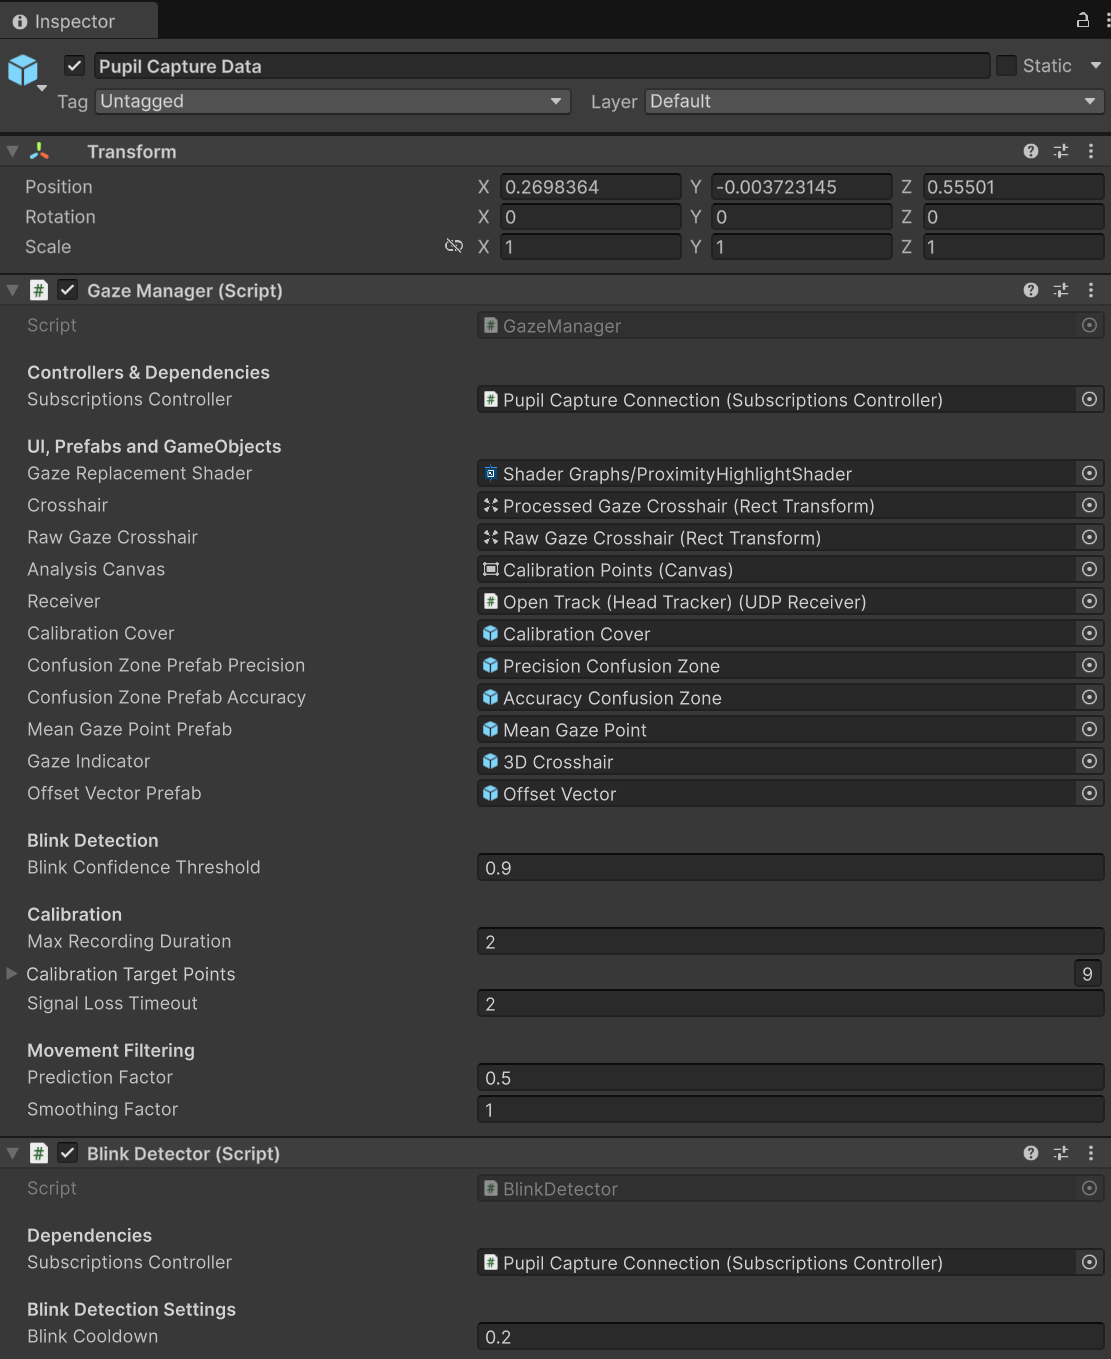
\includegraphics[width=0.4\linewidth]{images/gaze_manager.png}
    \caption{Paramètres de \texttt{Pupil Capture Data} à utiliser}
    \label{fig:gaze_manager}
\end{figure}
Dans la section \texttt{UI, Prefabs and GameObjects}, il suffit de suivre la même configuration. Cependant, les autres champs où il y a des valeurs à modifier, ces dernières peuvent être modifiée. Lire la documentation technique pour plus d'information.

\subsection{Calibration secondaire dans \texttt{Unity}}
Si les résultats de la calibration dans Pupil Capture ne sont pas satisfaisant, alors une calibration secondaire est possible dans \texttt{Unity}.
Cette calibration se passe en plusieurs étapes:
\begin{enumerate}
    \item Initialisation de la calibration : Appuyer sur le bouton \texttt{Calibration} dans la scène afin d'afficher un écran noir pour diminuer les distractions visuelles;
    \item Appuyer sur la touche \texttt{S} : Pour afficher la première cible de calibration, la calibration n'a pas encore commencé;
    \item Une fois que le regard est fixé sur la cible, appuyer sur la touche \texttt{R} : afin d'enregistrer les positions du regard par rapport à la cible en question : application de l'effet fenêtre virtuelle.
    \item Il faut refaire ces deux précédentes étapes sur les neufs points de calibration: une fois les neufs points effectué, la calibration est terminé.
    \item Appuyer sur la touche \texttt{N} pour appliquer la calibration est afficher les résultats à l'écran: on voit les vecteurs d'offset à chaque point de calibration et la zone de confusion qui change par rapport à la calibration.
    \item Pour enlever la visualisation des résultats de la calibration, appuyer sur la touche \texttt{V} : après cela, vous pouvez refaire une calibration en appuyant sur la touche \texttt{S} et refaire les étapes, ou bien revenir sur la scène en appuyant sur le bouton \texttt{Calibration}.
    \end{enumerate}
\begin{figure}[H]
    \centering
    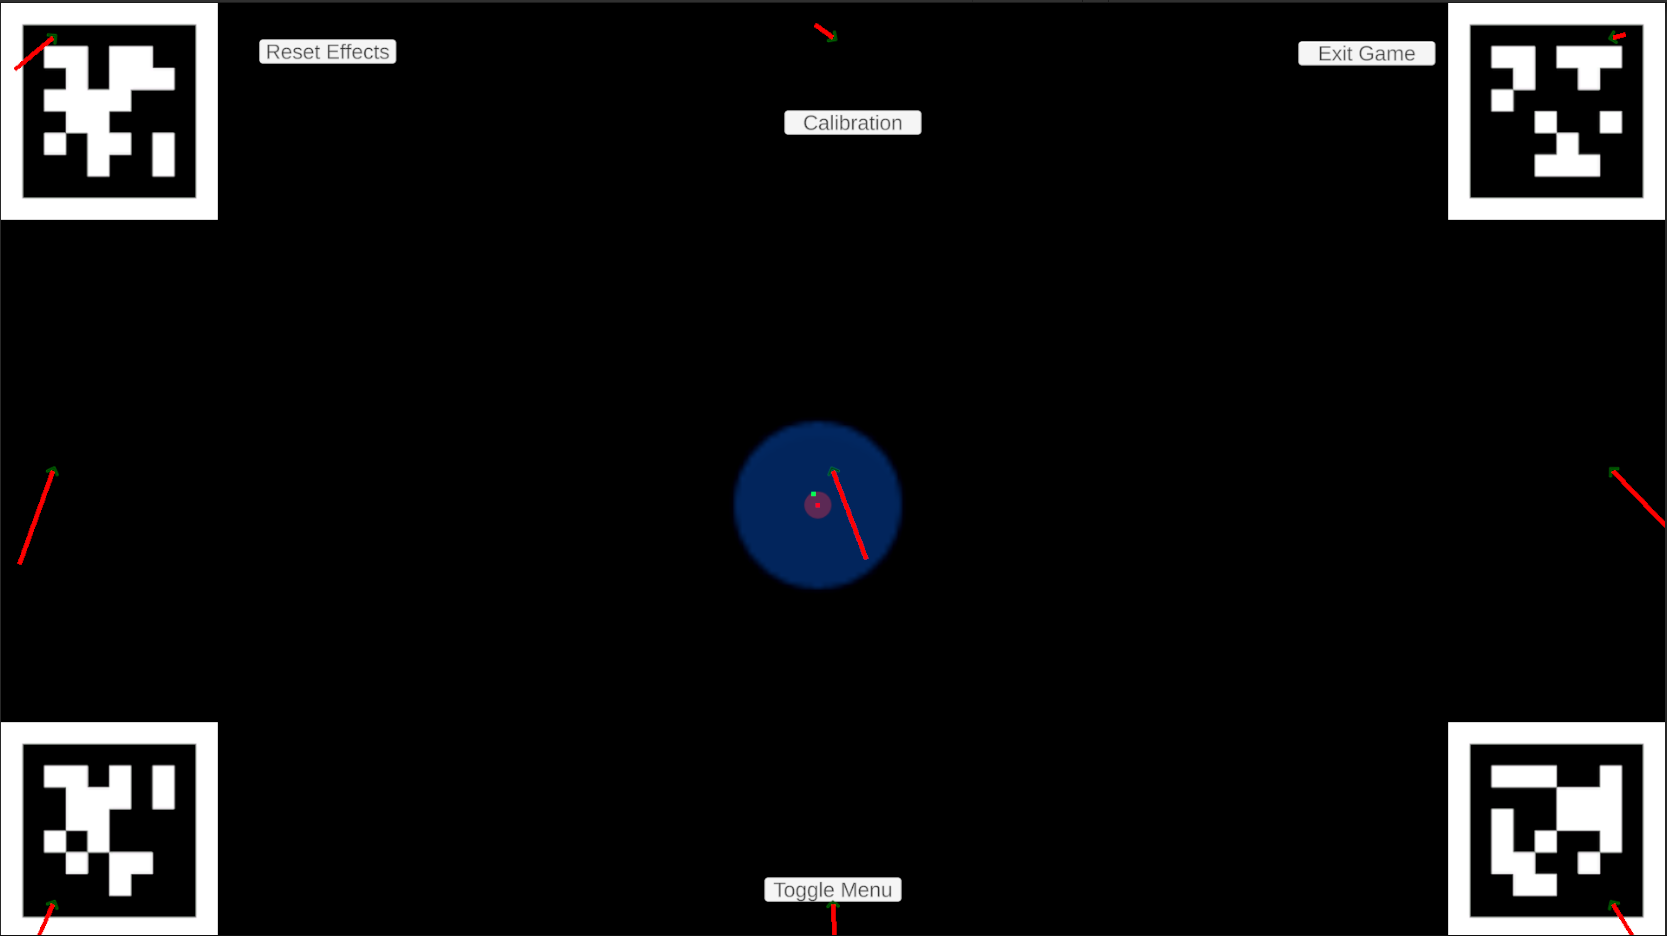
\includegraphics[width=0.8\linewidth]{images/calibration.png}
    \caption{Illustration des résultats de la calibration dans \texttt{Unity}}
    \label{fig:calibration}
\end{figure}
    

\chapter{Head-tracking}
\section{Présentation générale}
Le système de head-tracking permet à l'utilisateur d'explorer dynamiquement la scène 3D en bougeant sa tête. Il utilise un dispositif infrarouge avec des marqueurs placés sur un support métallique pouvant être attaché à un casque porté par l'utilisateur pour capturer les mouvements en temps réel. Ces mouvements sont envoyés via le réseau sous forme de position et, comme la version d'OpenTrack utilisée est modifiée, le nombre de points infrarouges couramment capturés est aussi récupérable. Ces informations permettent de réaliser un certain nombre de calculs permettant d'obtenir un effet de fenêtre physique sur un monde virtuel.

\begin{figure}[H]
    \centering
    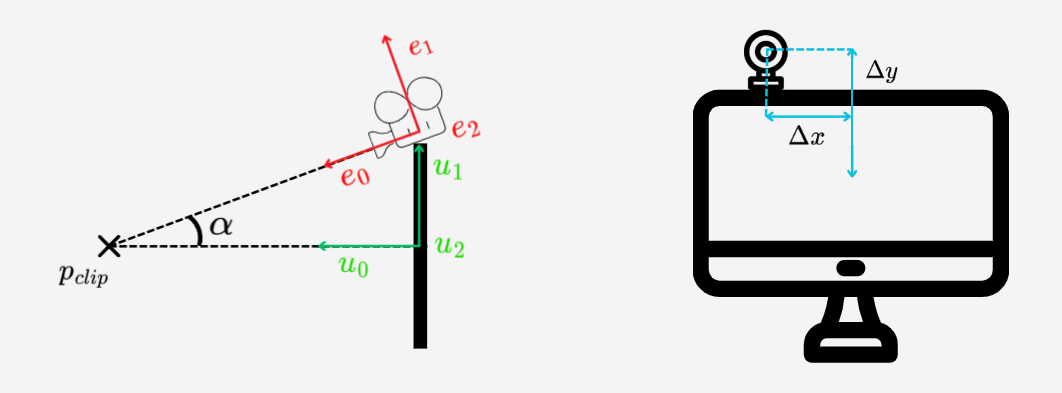
\includegraphics[width=0.8\textwidth]{images/headtracker/schema.png}
    \caption{Schéma du système de head-tracking avec dispositif infrarouge pris d'une diapositive de la présentation du prototype à l'équipe Manao. A gauche, un schéma illustrant la transformation nécessaire pour passer de la base caméra (rouge) à la base centre de l'écran (verte). Elle nécessite de connaître l'angle alpha et les offsets x et y en centimètres (vus sur le schéma de droite) qui peuvent être mis dans l'inspecteur pour qu'elle soit appliquée dans le code en recevant les données.}
    \label{fig:headtracking_schema}
\end{figure}

\section{Configuration et installation}
\subsection{Composants nécessaires}
\begin{itemize}
    \vspace{2mm}
    \item OpenTrack dont une version modifiée est fournie dans le dossier du projet. Il est situé dans \texttt{Opentrack/build/install/opentrack.exe};
    \vspace{2mm}
    \item caméra infrarouge;
    \vspace{2mm}
    \item leds infrarouges à placer sur un casque ou support.
    \vspace{2mm}
\end{itemize}

\subsection{Reconstruction depuis les sources}
Cette partie explique comment reconstruire Opentrack à partir du code source inclus avec le projet si des modifications venaient à être effectuées à ce dernier.
\subsubsection{Prérequis}

\begin{itemize}
    \vspace{2mm}
    \item \texttt{MSYS2 (64-bit)} avec la chaîne d'outils \texttt{MinGW-w64}. Le package \texttt{mingw-w64-x86\_64-qt5} est également nécessaire et peut être installé avec l'invité de commande \texttt{MSYS2 MinGW 64-bit} via la commande :
    \begin{lstlisting}[language=bash]
    pacman -S mingw-w64-x86_64-qt5
    \end{lstlisting}
    \vspace{2mm}
    \item \texttt{OpenCV} compatible avec la chaîne d'outils \texttt{MinGW}. Un dossier contenant le projet compilé pour la suite \texttt{MinGW} est disponible sur GitHub via \url{https://github.com/huihut/OpenCV-MinGW-Build};
    \vspace{2mm}
    \item \texttt{CMake} et \texttt{CMake GUI}.
    \vspace{2mm}
\end{itemize}

Il faut ajouter \texttt{C:\textbackslash msys64\textbackslash mingw64\textbackslash bin} au PATH système pour accéder aux outils \texttt{Qt} et \texttt{mingw32-make}.

\subsubsection{Configuration CMake}
\begin{itemize}
    \item configuration dans \texttt{CMake GUI} :
    \begin{itemize}
        \item source : chemin vers le dossier \texttt{OpenTrack} du projet;
        \item build : chemin vers le dossier \texttt{OpenTrack\_src/build} du projet;
        \item générateur : \texttt{"MinGW Makefiles"}.
    \end{itemize}
    
    \item variables essentielles :
    \begin{itemize}
        \item \texttt{CMAKE\_MAKE\_PROGRAM} $\rightarrow$ \texttt{C:/msys64/mingw64/bin/mingw32-make.exe};
        \item \texttt{OpenCV\_DIR} $\rightarrow$ dossier contenant \texttt{OpenCVConfig.cmake};
        \item \texttt{WITH\_OPENCV} = ON;
        \item \texttt{OPENTRACK\_PLUGIN\_INPUT\_PT} = ON.

        \begin{figure}[H]
            \centering
            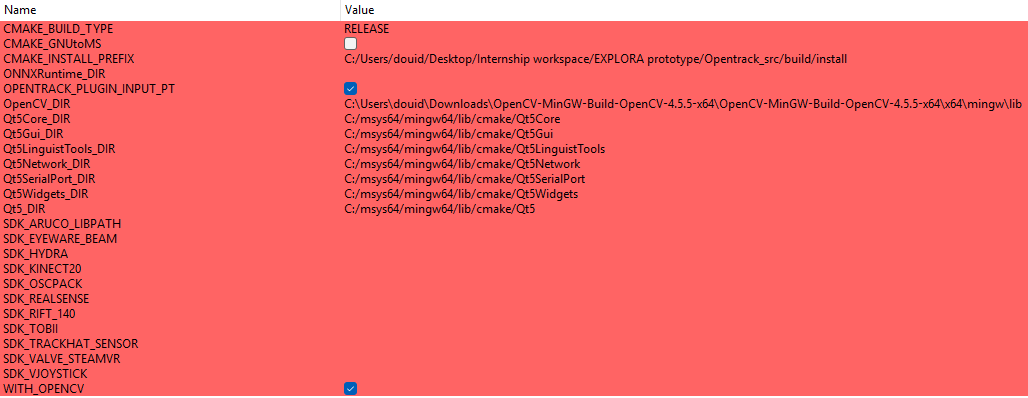
\includegraphics[width=0.99\textwidth]{images/headtracker/cmake_gui.png}
            \caption{Variables de compilation nécessaires dans \texttt{CMake GUI}. La plupart d'entre elles sont automatiquement prises en compte, mais certaines, décrites précédemment, doivent être manuellement créées.}
            \label{fig:cmake_variables}
        \end{figure}
    \end{itemize}
    
    \item commande de build et d'installation à exécuter dans un invité de commande depuis le dossier \texttt{/build} \textbf{APRÈS} avoir généré le projet en appuyant sur \texttt{Generate} en bas de la fenêtre d'application de \texttt{CMake GUI} :
    \begin{lstlisting}[language=bash]
    cmake --build . --target install
    \end{lstlisting}
\end{itemize}

L'installation génère dans \texttt{Opentrack/build/install/} l'exécutable et les DLL nécessaires à son fonctionnement.

\section{Paramétrage dans Opentrack}
Le paramétrage dans Opentrack se fait en premier lieu avec le profil en \texttt{.ini} fourni par les constructeurs de la caméra et du support à leds infrarouges. Ce profil, sous la forme d'un fichier nommé \texttt{Delanclip Starter - Metal Clip}, est fourni avec le projet dans le dossier \texttt{Opentrack/} et doit être sélectionné dans le champ \textit{Profile} de l'application. Les deux autres champs primordiaux sont :

\begin{itemize}
    \vspace{2mm}
    \item \textit{Input} : dans lequel on choisit le plugin \texttt{PointTracker 1.1}.
    \vspace{2mm}
    \item \textit{Output} : dans lequel on choisit \texttt{UDP over network}. C'est la méthode chargée d'envoyer sur les réseau les paquets devant être réceptionnés par \texttt{Unity}. En cliquant sur le marteau à droite de la méthode, il est possible de choisir l'adresse IPv4 à laquelle envoyer les paquets ainsi que le port. Si Opentrack et \texttt{Unity} sont exécutés sur le même ordinateur, alors il suffit de mettre l'adresse de \textit{loopback} 127.0.0.1. Sinon, il faut que l'ordinateur se chargeant des données et celui faisant tourner \texttt{Unity} soit sur le même réseau pour éviter les problématiques de pare-feu.
    \vspace{2mm}
\end{itemize}

\begin{figure}[H]
    \centering
    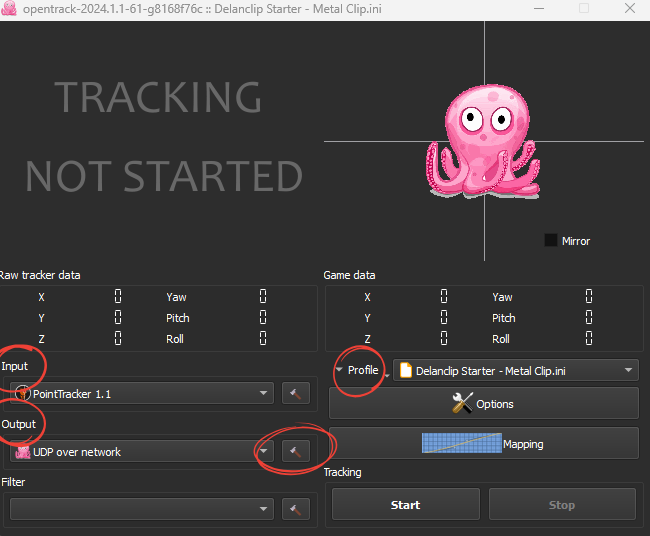
\includegraphics[width=0.8\textwidth]{images/headtracker/1.png}
    \caption{Fenêtre Opentrack sur laquelle sont entourés les champs de paramétrage évoqués.}
    \label{fig:opentrack_home}
\end{figure}

Comme on récupère les données brutes, dont la position donnée en centimètres par rapport à la caméra, et qu'on applique un léger filtrage de bruit par interpolation linéaire dans \texttt{Unity}, le champ \textit{Filter} ne sélectionne aucune méthode de filtrage. Par ailleurs, l'avatar de visualisation de la position et de la rotation de la tête par rapport à la caméra ne fonctionne pas dans cette version modifiée du logiciel, car la nature des données en sortie est différente de la version originale.

\section{Opentrack dans \texttt{Unity}}

Le système de head-tracking dans \texttt{Unity} repose sur trois composants principaux qui fonctionnent ensemble pour créer l'effet de fenêtre virtuelle.

\subsection{Architecture générale du système}

Le flux de données suit cette séquence (en utilisant le nom des classes appropriées) :
\begin{enumerate}
    \item \texttt{UDPReceiver} : réception et transformation des données brutes d'Opentrack;
    \item \texttt{HeadPositionController} : lissage et continuation de mouvement;
    \item \texttt{CameraController} : application de l'effet fenêtre virtuelle.
\end{enumerate}

\subsection{UDPReceiver}

\subsubsection{GameObject et rôle}
L'\texttt{UDPReceiver} est attaché à un GameObject vide nommé \textit{Open Track (Head Tracker)}. Ce composant constitue le point d'entrée des données du head-tracking dans \texttt{Unity}.

\subsubsection{Paramètres configurables dans l'inspecteur}

\begin{itemize}
    \vspace{2mm}
    \item \textbf{Transformation Settings} :
    \begin{itemize}
        \item \texttt{Scale Factor} : facteur d'échelle appliqué aux coordonnées reçues (par défaut : 0.01f);
        \item \texttt{X Rotation Angle Deg} : angle de rotation en degrés autour de l'axe X pour l'alignement des coordonnées (par défaut : 0.0f);
        \item \texttt{Translation} : offsets de translation pour appliquer une transformation de la base caméra à la base centre de l'écran vue sur la figure \ref{fig:headtracking_schema}  (par défaut : Vector2.zero).
    \end{itemize}
    \vspace{2mm}
    \item \textbf{Network Settings} :
    \begin{itemize}
        \item \texttt{Port} : port UDP pour la réception des données (par défaut : 4242). \textbf{Cependant ce paramètre ne fonctionne pas car le port est noté à la main dans la méthode chargée de la connection à la suite d'erreurs répétées}.
    \end{itemize}
    \vspace{2mm}
\end{itemize}

\begin{figure}[H]
    \centering
    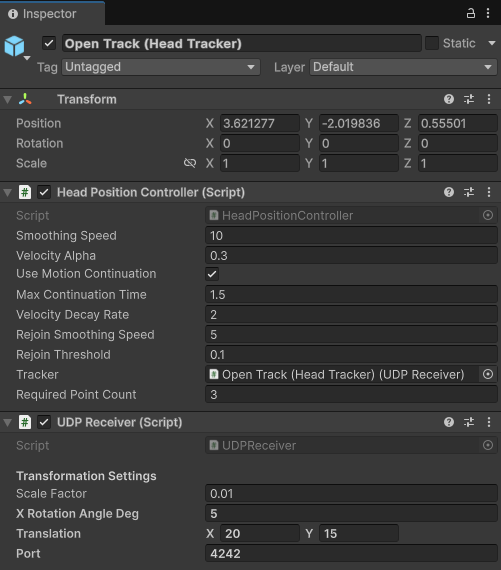
\includegraphics[width=0.6\textwidth]{images/headtracker/opentrack.png}
    \caption{Configuration du UDPReceiver et HeadPositionController dans l'inspecteur \texttt{Unity}.}
    \label{fig:udp_receiver_inspector}
\end{figure}

\subsection{HeadPositionController}

\subsubsection{GameObject et rôle}
Le \texttt{HeadPositionController} est attaché au même GameObject que \texttt{UDPReceiver}. Il fournit le lissage des données et la continuité de mouvement en cas de perte de signal.

\subsubsection{Paramètres configurables dans l'inspecteur}

\begin{itemize}
    \vspace{2mm}
    \item \textbf{Smoothing Settings} :
    \begin{itemize}
        \item \texttt{Smoothing Speed} : vitesse d'interpolation de position pendant le suivi normal (par défaut : 10f);
        \item \texttt{Velocity Alpha} : facteur de lissage exponentiel pour l'estimation de vitesse (0-1, par défaut : 0.3f).
    \end{itemize}
    \vspace{2mm}
    \item \textbf{Motion Continuation} :
    \begin{itemize}
        \item \texttt{Use Motion Continuation} : active la continuation prédictive lors de la perte de signal (par défaut : true);
        \item \texttt{Max Continuation Time} : durée maximale de prédiction de mouvement (par défaut : 1.5f secondes);
        \item \texttt{Velocity Decay Rate} : taux de décroissance exponentielle de la vitesse (par défaut : 2f).
    \end{itemize}
    \vspace{2mm}
    \item \textbf{Rejoining Settings} :
    \begin{itemize}
        \item \texttt{Rejoin Smoothing Speed} : vitesse de lissage lors de la reconnexion (par défaut : 5f);
        \item \texttt{Rejoin Threshold} : seuil de distance pour sortir du mode reconnexion (par défaut : 0.1f).
    \end{itemize}
    \vspace{2mm}
    \item \textbf{Tracker Settings} :
    \begin{itemize}
        \item \texttt{Tracker} : référence vers le composant UDPReceiver;
        \item \texttt{Required Point Count} : nombre minimum de points requis pour un suivi valide (par défaut : 3).
    \end{itemize}
    \vspace{2mm}
\end{itemize}

\subsection{CameraController}

\subsubsection{GameObject et rôle}
Le \texttt{CameraController} doit être attaché au GameObject de la caméra principale (\textit{Main Camera}). Il applique l'effet de fenêtre virtuelle en ajustant dynamiquement la position, l'orientation et le champ de vision de la caméra.

\subsubsection{Paramètres configurables}

\begin{itemize}
    \vspace{2mm}
    \item \textbf{Head Tracking Reference} :
    \begin{itemize}
        \item \texttt{Head Position} : référence vers le composant HeadPositionController qui fournit les données de position lissées
    \end{itemize}
    \vspace{2mm}
\end{itemize}

\begin{figure}[H]
    \centering
    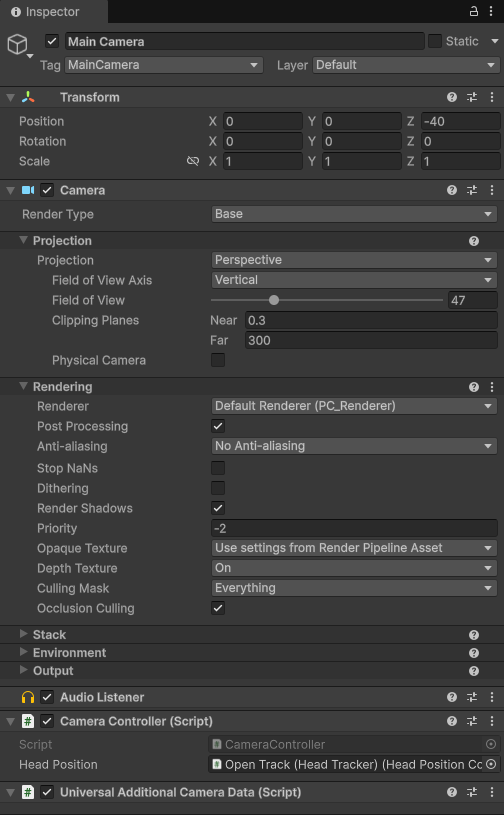
\includegraphics[width=0.4\textwidth]{images/headtracker/main_camera.png}
    \caption{Configuration du CameraController dans l'inspecteur \texttt{Unity}}
    \label{fig:camera_controller_inspector}
\end{figure}

\chapter{Cécité au changement}
\section{Présentation générale}
Le système de cécité au changement (ou \textit{change blindness}) permet de réaliser des expériences de cécité au changement dans l'environnement virtuel \texttt{Unity}. Ce phénomène psychologique consiste en l'incapacité des observateurs à détecter des changements visuels significatifs lorsque ceux-ci se produisent pendant une interruption visuelle ou en dehors du champ de vision direct. Le système implémenté supporte deux types d'expériences principales (correspondant à une énumération dans le code, détaillée dans la documentation technique du projet) et est en partie basé sur les travaux de \textit{Martin et al.}~\cite{10049723} :

\begin{itemize}
    \vspace{2mm}
    \item \texttt{InFoV} \textit{(In Field of View)} : les changements se produisent lorsque l'objet est dans le champ de vision et que le regard de l'utilisateur est dirigé vers l'objet cible, généralement pendant un clignement d'œil pour masquer le changement ;
    \vspace{2mm}
    \item \texttt{OutFoV} \textit{(Out of Field of View)} : les changements se produisent lorsque l'objet est en dehors du champ de vision de l'utilisateur, créant une surprise lorsque celui-ci reporte son attention sur la zone modifiée.
    \vspace{2mm}
\end{itemize}

\section{Architecture du système}
\subsection{Composants principaux}
Le système de change blindness est organisé autour de plusieurs composants clés :

\begin{itemize}
    \vspace{2mm}
    \item \texttt{ChangeBlindnessManager} : classe implémentant un gestionnaire central qui coordonne toutes les expériences et déclenche les changements selon les conditions définies ;
    \vspace{2mm}
    \item \texttt{IExperiment} : interface définissant les capacités requises pour qu'un objet puisse participer aux expériences ;
    \vspace{2mm}
    \item \texttt{BaseExperiment} : classe abstraite de base fournissant les fonctionnalités communes à tous les types d'expériences ;
    \vspace{2mm}
    \item des expériences spécialisées : classes implémentant des types de changements spécifiques (couleur, position, échange d'objets, etc.).
    \vspace{2mm}
\end{itemize}

\subsection{Configuration du ChangeBlindnessManager}
Le \texttt{ChangeBlindnessManager} constitue le cœur du système et doit être configuré dans l'inspecteur \texttt{Unity} avec les paramètres suivants :

\begin{itemize}
    \vspace{2mm}
    \item \texttt{Main Camera} : référence vers la caméra principale utilisée pour les calculs de champ de vision ;
    \vspace{2mm}
    \item \texttt{Experiments} : liste de toutes les expériences (correspondant à un objet \texttt{Unity} vide auquel est attaché le script associé à l'expérience voulue) qui pourront être déclenchées lors du lancement de la scène ;
    \vspace{2mm}
    \item \texttt{Min Time Between Changes} : intervalle minimum (en secondes) devant s'écouler entre deux changements consécutifs  ;
    \vspace{2mm}
    \item \texttt{Start Experiment Button} et \texttt{Reset Button} : boutons UI pour le contrôle de l'expérience.
    \vspace{2mm}
\end{itemize}

\begin{figure}[H]
    \centering
    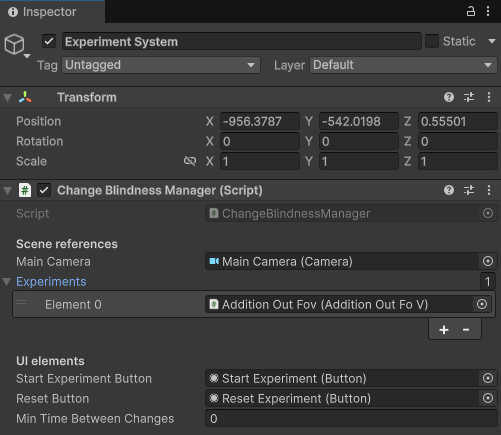
\includegraphics[width=0.6\textwidth]{images/changeblindness/manager.png}
    \caption{Configuration du ChangeBlindnessManager dans l'inspecteur \texttt{Unity}}
    \label{fig:manager_inspector}
\end{figure}

\section{Exemples d'expériences disponibles}

Pour rappel, ces expériences sont créées sous la forme d'un objet \texttt{Unity} auquel est attaché le script de cette dernière.

\subsection{Expériences InFoV}

Les expériences InFoV se déclenchent lorsque l'objet est visible dans le champ de vision et que l'utilisateur réalise une action déclencheuse (porter son regard vers un objet cible en utilisant le cercle de confusion, cligner des yeux, etc.).

\subsubsection{ColorInFoV}
Change la couleur d'un objet de manière aléatoire lorsque l'utilisateur le regarde directement. Les paramètres configurables sont :
\begin{itemize}
    \vspace{2mm}
    \item \texttt{Object To Observe} : l'objet qui doit être observé pour déclencher le changement de couleur ;
    \vspace{2mm}
    \item \texttt{Target Object To Change} : l'objet dont la couleur sera modifiée.
    \vspace{2mm}
\end{itemize}

\subsection{Expériences OutFoV}

Les expériences OutFoV se déclenchent lorsque le/les objet(s) cible(s) est/sont en dehors du champ de vision de l'utilisateur.

\subsubsection{MovementOutFoV}
Déplace un objet vers une nouvelle position lorsqu'il est hors du champ de vision. Les paramètres configurables sont :
\begin{itemize}
    \vspace{2mm}
    \item \texttt{Changed Position} : la nouvelle position dans l'espace monde où l'objet sera déplacé ;
    \vspace{2mm}
    \item \texttt{Target Object} : l'objet qui sera déplacé pendant l'expérience.
    \vspace{2mm}
\end{itemize}

\begin{figure}[h!]
    \centering
    \begin{subfigure}[b]{0.485\textwidth}
        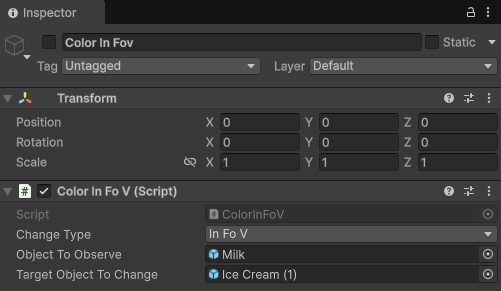
\includegraphics[width=\textwidth]{./images/changeblindness/color_in_fov}
        \caption{\footnotesize Color in FoV experiment.}
        \label{fig:colorinfov}
    \end{subfigure}
    \begin{subfigure}[b]{0.489\textwidth}
        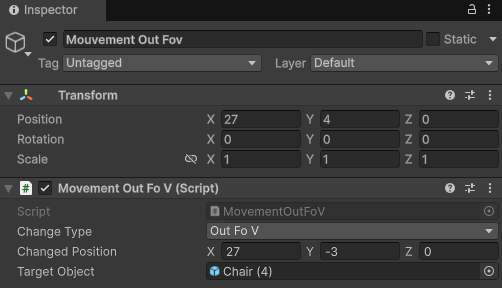
\includegraphics[width=\textwidth]{./images/changeblindness/move_out_fov}
        \caption{\footnotesize Movement out FoV experiment.}
        \label{fig:movoutfov}
    \end{subfigure}
    \caption{Les deux expériences données en exemple vues depuis l'inspecteur \texttt{Unity}.}
    \label{fig:experiences_exemple}
\end{figure}

\section{Ajout d'expériences personnalisées}

\subsection{Création d'une nouvelle expérience}

Pour créer une nouvelle expérience de \textit{change blindness}, il faut :

\begin{enumerate}
    \item créer une nouvelle classe héritant de \texttt{BaseExperiment} ;
    \item implémenter les méthodes abstraites requises ;
    \item configurer l'objet dans l'inspecteur \texttt{Unity} ;
    \item l'ajouter à la liste des expériences du \texttt{ChangeBlindnessManager}.
\end{enumerate}

\subsection{Méthodes à implémenter}

Toute expérience personnalisée doit implémenter les méthodes suivantes :
\vspace{2mm}

{\small
\begin{lstlisting}
public override void ApplyChange()
{
    // Logique pour appliquer le changement
    // Marquer IsChanged = true
}

public override void RevertChange()
{
    // Logique pour annuler le changement
    // Marquer IsChanged = false
}

public override bool IsInFieldOfView(Camera camera)
{
    // Logique pour determiner si l'objet est visibile
    // Retourner true/false selon la visibilite
}
\end{lstlisting}
}

\subsection{Exemple d'implémentation}

Voici un exemple d'implémentation d'une expérience personnalisée qui modifie la taille d'un objet :
\vspace{2mm}

{\small
\lstset{style=sharpc}
\begin{lstlisting}
public class ScaleChangeInFoV : BaseExperiment
{
    [SerializeField] private GameObject targetObject;
    [SerializeField] private Vector3 newScale = Vector3.one * 2f;
    private Vector3 originalScale;
    
    private void Start()
    {
        originalScale = targetObject.transform.localScale;
    }
    
    public override void ApplyChange()
    {
        targetObject.transform.localScale = newScale;
        IsChanged = true;
    }
    
    public override void RevertChange()
    {
        targetObject.transform.localScale = originalScale;
        IsChanged = false;
    }
    
    public override bool IsInFieldOfView(Camera camera)
    {
        Vector3 screenPoint = 
                camera.WorldToViewportPoint(
                    targetObject.transform.position);
        bool isGazeOnTarget = 
                IsObjectToObserveInConfusionCircle(targetObject, 
                                                    camera);
        bool isVisible = screenPoint.z > 0 && 
                         screenPoint.x > 0 && screenPoint.x < 1 && 
                         screenPoint.y > 0 && screenPoint.y < 1;
        
        return isGazeOnTarget && isVisible;
    }
}
\end{lstlisting}
}

\section{Gestion et intégration}

\subsection{Gestion de l'état}
Le système maintient un état global qui comprend :
\begin{itemize}
    \item l'état d'activation de l'expérience (\texttt{isExperimentRunning}) ;
    \item la liste des objets ayant déjà été modifiés (\texttt{activeChanges}) ;
    \item le timestamp du dernier changement pour respecter l'intervalle minimum entre les modifications.
\end{itemize}

\subsection{Intégration avec l'eye-tracking}

Le système s'intègre automatiquement avec les composants d'eye-tracking disponibles dans la scène :
\begin{itemize}
    \vspace{2mm}
    \item \texttt{GazeManager} : pour obtenir la position du regard et le rayon de précision ;
    \vspace{2mm}
    \item \texttt{BlinkDetector} : pour détecter les clignements d'œil et déclencher les changements pendant ces moments d'occultation naturelle.
    \vspace{2mm}
\end{itemize}

\chapter{Système d'illusions visuelles}
\section{Présentation générale}
Le système d'illusions visuelles permet de créer et contrôler des effets de post-processing en temps réel dans l'environnement \texttt{Unity}, en se basant sur les données de suivi oculaire et de position de tête de l'utilisateur. Ce système implémente diverses illusions perceptuelles qui s'adaptent dynamiquement au comportement visuel de l'utilisateur, créant des expériences immersives et interactives.

Le système supporte plusieurs types d'effets visuels (correspondant à une énumération dans le code) :

\begin{itemize}
    \vspace{2mm}
    \item \texttt{DepthOfField} : simulation de profondeur de champ photographique basée sur les zones de confusion de regard ;
    \vspace{2mm}
    \item \texttt{Vignette} : effet de vignettage dynamique qui suit le regard de l'utilisateur ;
    \vspace{2mm}
    \item \texttt{ChromaticAberration} : aberration chromatique variable selon l'excentricité du regard ;
    \vspace{2mm}
    \item \texttt{Bloom} : effet de surbrillance adaptatif basé sur la profondeur de regard ;
    \vspace{2mm}
    \item \texttt{LensDistortion} : distortion de lentille dynamique centrée sur le point de regard ;
    \vspace{2mm}
    \item \texttt{DirectionalLightRotation} : rotation de l'éclairage directionnel basée sur les mouvements de tête.
    \vspace{2mm}
\end{itemize}

\section{Architecture du système}
\subsection{Composants principaux}
Le système d'illusions visuelles est organisé autour de trois composants clés :

\begin{itemize}
    \vspace{2mm}
    \item \texttt{EffectsManager} : gestionnaire central qui coordonne les effets visuels et gère l'état de l'interface utilisateur ;
    \vspace{2mm}
    \item \texttt{PostProcessManager} : contrôleur technique des effets de post-processing et de leurs paramètres en temps réel ;
    \vspace{2mm}
    \item \texttt{IllusionUI} : interface utilisateur pour la sélection et le contrôle des effets visuels.
    \vspace{2mm}
\end{itemize}

\subsection{Configuration de l'EffectsManager}
L'\texttt{EffectsManager} constitue le point d'entrée principal du système et doit être configuré dans l'inspecteur \texttt{Unity} avec les paramètres suivants :

\begin{itemize}
    \vspace{2mm}
    \item \texttt{Post Process Manager} : référence vers le gestionnaire technique des effets (auto-assigné si sur le même GameObject) ;
    \vspace{2mm}
    \item \texttt{Effects Panel} : panneau UI contenant les contrôles des effets, masqué automatiquement lors de l'activation des effets.
    \vspace{2mm}
\end{itemize}

\subsection{Configuration du PostProcessManager}
Le \texttt{PostProcessManager} est le cœur technique du système et nécessite une configuration plus détaillée :

\begin{itemize}
    \vspace{2mm}
    \item \texttt{Volume} : volume \texttt{Unity} contenant le profil des effets de post-processing ;
    \vspace{2mm}
    \item \texttt{Main Camera} : caméra principale pour les calculs de profondeur et les effets basés sur la vue ;
    \vspace{2mm}
    \item \texttt{Gaze Detector} : système de détection du regard fournissant les données d'attention ;
    \vspace{2mm}
    \item \texttt{Smooth Speed} : facteur de lissage pour les transitions graduelles des effets ;
    \vspace{2mm}
    \item \texttt{Depth Confusion Zone Analyser} : analyseur fournissant les données de plage de profondeur pour les calculs de mise au point ;
    \vspace{2mm}
    \item \texttt{Directional Light} : lumière directionnelle principale pour les effets d'éclairage dynamique ;
    \vspace{2mm}
    \item paramètres spécifiques aux effets expliqués dans la documentation technique : intensités, seuils, vitesses de transition, etc.
    \vspace{2mm}
\end{itemize}

\begin{figure}[H]
    \centering
    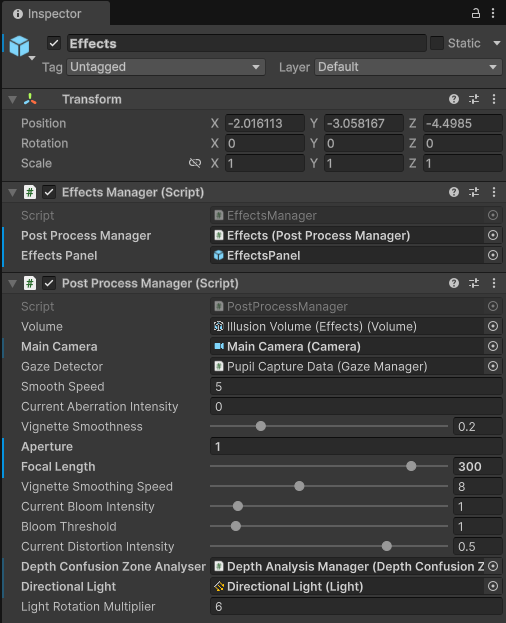
\includegraphics[width=0.5\textwidth]{images/changeblindness/postprocess.png}
    \caption{Configuration du PostProcessManager dans l'inspecteur \texttt{Unity}}
    \label{fig:postprocess_inspector}
\end{figure}

\section{Effets disponibles}

\subsection{Profondeur de champ (DepthOfField)}
Simule une profondeur de champ photographique réaliste en utilisant les principes optiques. L'effet calcule automatiquement :
\begin{itemize}
    \vspace{2mm}
    \item la distance de mise au point basée sur la limite proche de la zone de confusion ;
    \vspace{2mm}
    \item la distance hyperfocale pour que la limite lointaine tombe dans la zone de netteté acceptable ;
    \vspace{2mm}
    \item l'ouverture requise utilisant les contraintes du cercle de confusion.
    \vspace{2mm}
\end{itemize}

Pour plus d'informations, il est possible de se reporter à la documentation technique et à l'implémentation elle-même.

\subsection{Vignettage dynamique (Vignette)}
Crée un effet de vignettage dont le centre suit le regard de l'utilisateur. Paramètres configurables :
\begin{itemize}
    \vspace{2mm}
    \item \texttt{Vignette Intensity} : intensité de l'assombrissement des bords ;
    \vspace{2mm}
    \item \texttt{Vignette Smoothness} : douceur de la transition des bords ;
    \vspace{2mm}
    \item \texttt{Vignette Smoothing Speed} : vitesse d'ajustement de la position du vignettage.
    \vspace{2mm}
\end{itemize}

\subsection{Aberration chromatique (ChromaticAberration)}
Applique une aberration chromatique variable selon l'excentricité du regard par rapport au centre de l'écran :
\begin{itemize}
    \vspace{2mm}
    \item l'intensité est inversement proportionnelle à la proximité du centre ;
    \vspace{2mm}
    \item \texttt{Current Aberration Intensity} : intensité actuelle appliquée à la simulation de lentille.
    \vspace{2mm}
\end{itemize}

\subsection{Effet de surbrillance (Bloom)}
Effet de surbrillance adaptatif basé sur la profondeur du regard :
\begin{itemize}
    \vspace{2mm}
    \item \texttt{Current Bloom Intensity} : intensité actuelle de l'effet de surbrillance ;
    \vspace{2mm}
    \item \texttt{Bloom Threshold} : seuil de luminosité au-dessus duquel l'effet s'active.
    \vspace{2mm}
\end{itemize}

\subsection{Distortion de lentille (LensDistortion)}
Distortion dynamique qui s'intensifie avec la distance du regard par rapport au centre :
\begin{itemize}
    \vspace{2mm}
    \item \texttt{Current Distortion Intensity} : intensité actuelle de la distortion ;
    \vspace{2mm}
    \item \texttt{Distortion Scale} : facteur d'échelle contrôlant la zone de couverture de l'effet.
    \vspace{2mm}
\end{itemize}

\section{Interface utilisateur}

\subsection{Configuration de l'IllusionUI}
L'\texttt{IllusionUI} gère les interactions utilisateur et doit être configuré avec :

\begin{itemize}
    \vspace{2mm}
    \item \texttt{Illusion Manager} : référence vers l'EffectsManager pour la délégation des commandes ;
    \vspace{2mm}
    \item \texttt{Effects Panel} : panneau UI contenant les boutons de contrôle des effets.
    \vspace{2mm}
\end{itemize}

Le système masque automatiquement les éléments de visualisation ("Visualization Elements" et "3D Crosshair") lors de l'activation des effets pour une démonstration propre.

\section{Ajout d'effets personnalisés}

\subsection{Création d'un nouvel effet}

Pour créer un nouvel effet de post-processing, il faut :

\begin{enumerate}
    \item Ajouter le nouvel effet à l'énumération \texttt{PostProcessEffect} ;
    \item Créer les champs de configuration appropriés dans \texttt{PostProcessManager} ;
    \item Implémenter la méthode de mise à jour de l'effet ;
    \item Ajouter l'effet aux dictionnaires d'initialisation.
\end{enumerate}

\subsection{Implémentation d'une méthode de mise à jour}

Toute méthode de mise à jour d'effet personnalisé doit suivre le pattern suivant :

{\small
\lstset{style=sharpc}
\begin{lstlisting}
private void UpdateCustomEffect()
{
    if (customEffect == null || gazeDetector == null) return;
    
    // Calculs bases sur les donnees de regard/tete
    Vector3 gazeWorld = gazeDetector.CurrentGazeHit.point;
    
    // Application des parametres avec lissage
    float targetValue = CalculateTargetValue(gazeWorld);
    currentValue = Mathf.Lerp(currentValue, targetValue, 
                             Time.deltaTime * smoothSpeed);
    
    // Application a l'effet de post-processing
    customEffect.parameter.value = currentValue;
}
\end{lstlisting}
}

\subsection{Intégration dans le système}

L'effet doit être ajouté aux dictionnaires situés dans la méthode \texttt{InitializeEffectDictionaries()} de la classe \texttt{PostProcessManager}. Il est nécessaire de l'ajouter au premier dictionnaire \texttt{effectsComponents} si c'est un effet intégré à \texttt{Unity} et qu'il possède son entrée dans le volume global de la scène.

\chapter{Analyseur de zones de regard (GazeAnalyzer)}
\section{Présentation générale}
Le système GazeAnalyzer permet d'analyser quantitativement la distribution du regard de l'utilisateur sur les objets présents dans la scène virtuelle. Il détermine quelle proportion de la zone de confusion du regard est occupée par chaque objet analysable.

Le système fonctionne en deux phases principales : une phase de segmentation par rendu d'identifiants colorés et une phase d'analyse proportionnelle des pixels dans la zone de regard circulaire. L'ensemble utilise un traitement asynchrone sur GPU et des threads en arrière-plan pour l'analyse.

Étant donné le passage à une représentation en trois dimensions de la zone de regard via la \textit{search light}, le système n'est pas utilisé dans le projet, mais l'objet \texttt{Unity} l'englobant est toujours présent dans l'inspecteur.

\section{Architecture du système}
\subsection{Composants principaux}
Le système GazeAnalyzer est composé de deux scripts complémentaires :

\begin{itemize}
    \vspace{2mm}
    \item \texttt{GazeZoneAnalyzer} : analyseur technique principal qui effectue la segmentation des objets et le calcul des proportions ;
    \vspace{2mm}
    \item \texttt{GazeProportionAnalyzer} : analyseur périodique qui interroge le système et rapporte les résultats significatifs.
    \vspace{2mm}
\end{itemize}

\subsection{Configuration du GazeZoneAnalyzer}
Le \texttt{GazeZoneAnalyzer} constitue le cœur technique du système et nécessite la configuration suivante dans l'inspecteur \texttt{Unity} :

\begin{itemize}
    \vspace{2mm}
    \item \texttt{Gaze Detector} : référence vers le système de détection du regard (GazeManager) ;
    \vspace{2mm}
    \item \texttt{Main Camera} : caméra principale utilisée comme référence pour la caméra de segmentation ;
    \vspace{2mm}
    \item \texttt{Parent Hierarchy} : objet parent depuis lequel peupler automatiquement la liste des objets analysables ;
    \vspace{2mm}
    \item \texttt{Analyzable Objects} : liste des GameObjects à analyser (peuplée automatiquement depuis la hiérarchie parent). Les objets formant l'arrière plan sont distingués dans le script par la présence de \textit{Background} dans leurs noms.
    \vspace{2mm}
\end{itemize}

\subsection{Configuration du GazeProportionAnalyzer}
Le \texttt{GazeProportionAnalyzer} gère l'analyse périodique et les rapports :

\begin{itemize}
    \vspace{2mm}
    \item \texttt{Gaze Zone Analyzer} : référence vers le GazeZoneAnalyzer fournissant les proportions par objet ;
    \vspace{2mm}
    \item \texttt{Analysis Interval} : intervalle de temps (en secondes) entre les analyses consécutives ;
    \vspace{2mm}
    \item \texttt{Minimum Proportion Threshold} : proportion minimale (0-1) requise pour considérer un objet comme significatif.
    \vspace{2mm}
\end{itemize}

\begin{figure}[H]
    \centering
    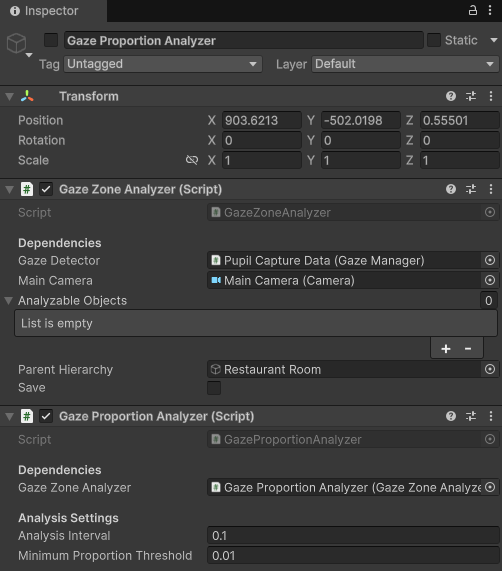
\includegraphics[width=0.6\textwidth]{images/headtracker/analyzer.png}
    \caption{Configuration du du GazeAnalyzer dans l'inspecteur \texttt{Unity}}
    \label{fig:proportion_analyzer}
\end{figure}

\section{Fonctionnement technique}

\subsection{Principe de segmentation par identifiants colorés}
Le système utilise une technique de segmentation avancée où chaque objet analysable se voit attribuer un identifiant unique encodé sous forme de couleur RGB. Une caméra de segmentation dédiée effectue un rendu spécialisé où chaque objet apparaît dans sa couleur d'identifiant, permettant une identification précise au niveau du pixel.

\subsection{Analyse de la zone de regard}
L'analyse se concentre sur la zone circulaire de confusion du regard, définie par le système de suivi oculaire. Le système compte les pixels de chaque couleur d'identifiant présents dans ce cercle et calcule la proportion relative occupée par chaque objet. 

\subsection{Traitement asynchrone}
Pour maintenir les performances, le système utilise :
\begin{itemize}
    \vspace{2mm}
    \item Lecture asynchrone GPU (\texttt{AsyncGPUReadback}) pour récupérer les données de pixels ;
    \vspace{2mm}
    \item Traitement en thread séparé pour l'analyse des pixels ;
    \vspace{2mm}
    \item Mise en cache des résultats pour éviter les blocages pendant le traitement.
    \vspace{2mm}
\end{itemize}

\subsection{Interprétation des résultats}
Les résultats sont fournis sous forme de dictionnaire associant chaque GameObject à sa proportion (valeur entre 0 et 1) de la zone de regard. Une proportion de 0.25 signifie que l'objet occupe 25\% de la zone de confusion du regard.

\chapter{Système de search light}
\section{Présentation générale}
Le système de search light nous permet de modéliser le problème de la zone de regard de façon à récupérer la profondeur minimum et maximum de la zone du regard avec un compute shader en premier lieu. Ce dernier nous permet de faire ça à l'aide du depth buffer envoyé par une camera secondaire.
Aussi, ce système nous permet de récupérer les fragments contenus dans la zone de regard, ce qui nous permet de modifier l'aspect visuel de ces fragments à notre guise.
\section{Changement des propriétés des matériaux}
Afin de modifier les propriétés des matériaux des objets qui nous intéressent, nous avons mis en place un système de shaders. Ce système est crée sur \texttt{Shader Graph}, qui nous permet de créer un vertex et un fragment shader sans difficulté et de modifier les entrées de ces dernier afin de changer les propriétés des fragments contenus dans la zone du regard. Actuellement, la seule propriété qu'on change est l’émissivité du matériau.
Cependant, pour des raisons de simplicité il faut créer et sélectionner des matériaux utilisant ce shader sur chaque object sur lequel on veut appliquer l'effet pour avoir une visualisation satisfaisante. Le shader en question est dans le dossier \texttt{assets/Resources/Shaders} nommé \texttt{ProximityHighlightShader}.
De ce fait, on peut créer de multiples shaders pour chaque effet en modifiant les propriétés des matériaux utilisés.
\begin{figure}[H]
    \centering
    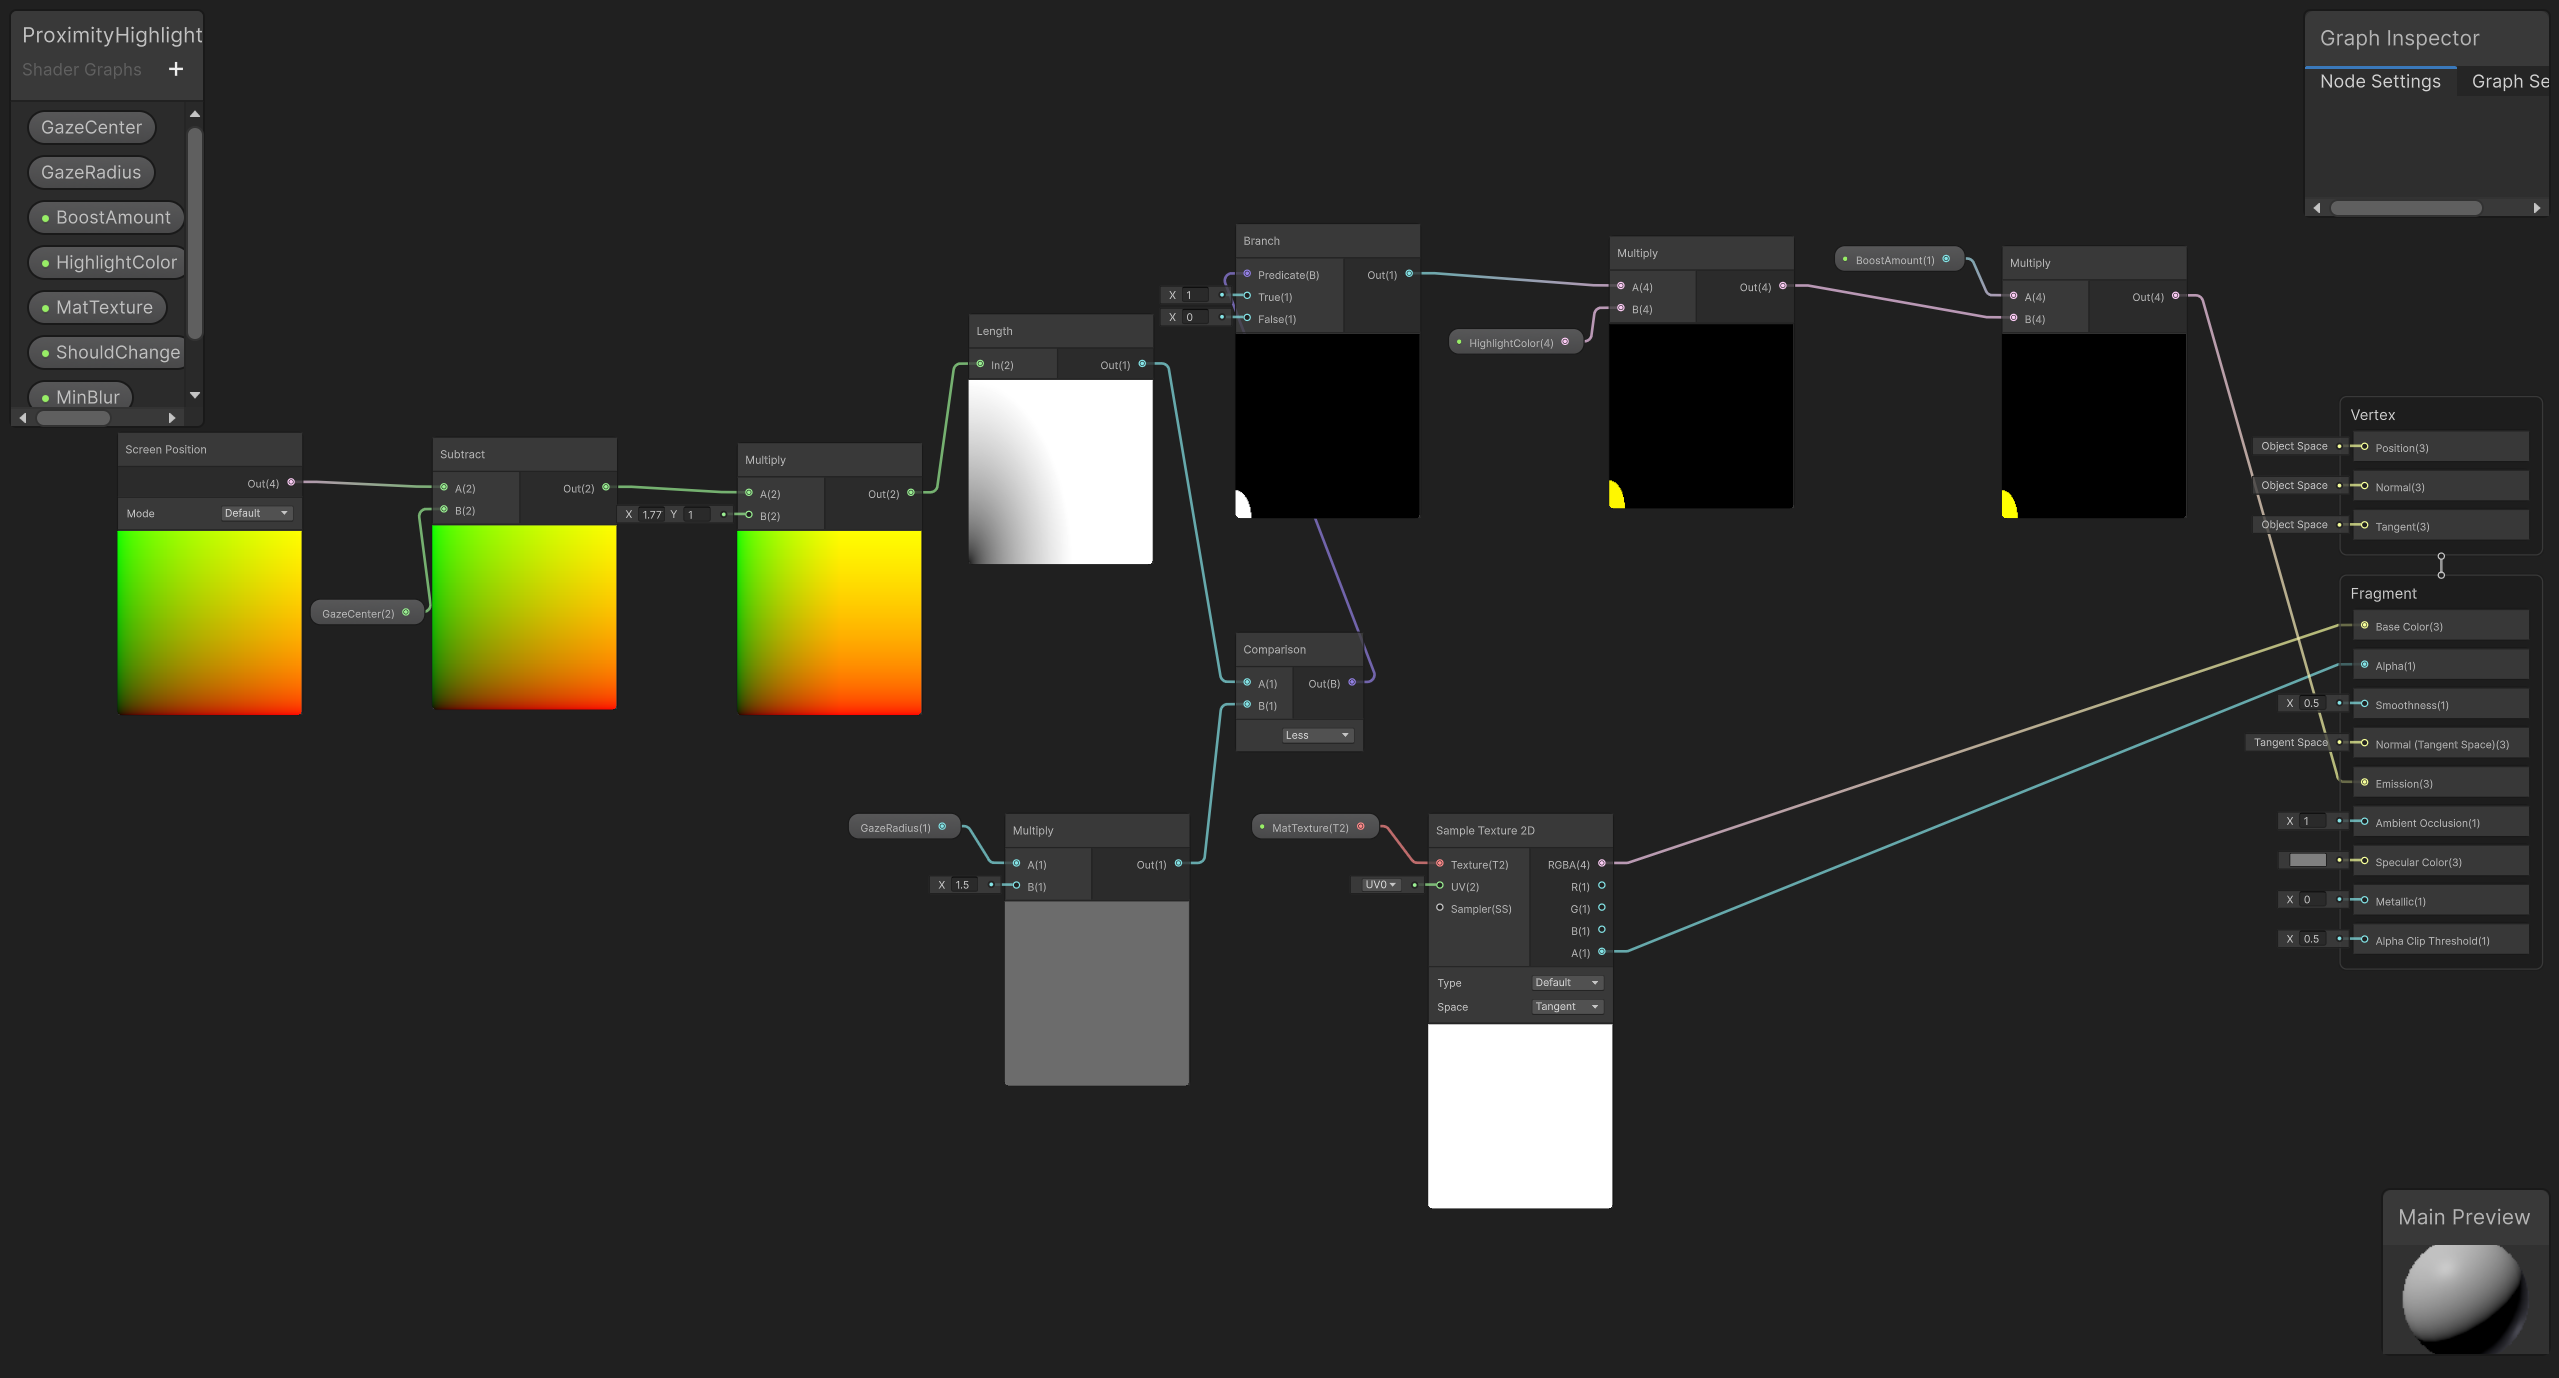
\includegraphics[width=0.8\linewidth]{images/shader_graph.png}
    \caption{Schéma du Lit \texttt{Shader Graph} utilisé pour avoir l'effet de search light sur les objets}
    \label{fig:shader_graph}
\end{figure}
\section{Profondeur minimum et maximum}
Pour certains effets, dont la profondeur de champ, l'information de la profondeur est crucial pour avoir un effet convaincant. Pour ce faire, un compute shader a été créé afin de calculer la profondeur minimum et maximum de la zone du regard utilisant le depth buffer d'une seconde camera nommée \texttt{depth camera}. Cette camera suivra la camera principale mais ne fera le rendu que des objets qui nous intéressent pour le calcul de la profondeur, donc tous sauf les murs, le plafond et le sol.
Pour configurer cela, il faut mettre les objets d'arrière plan dans une couche de rendu dédiée (la couche \texttt{background} dans notre scène), et configurer \texttt{depth camera} pour que le culling mask prend toutes les couches sauf la couche des objets en arrière plan.
\begin{figure}[H]
    \centering
    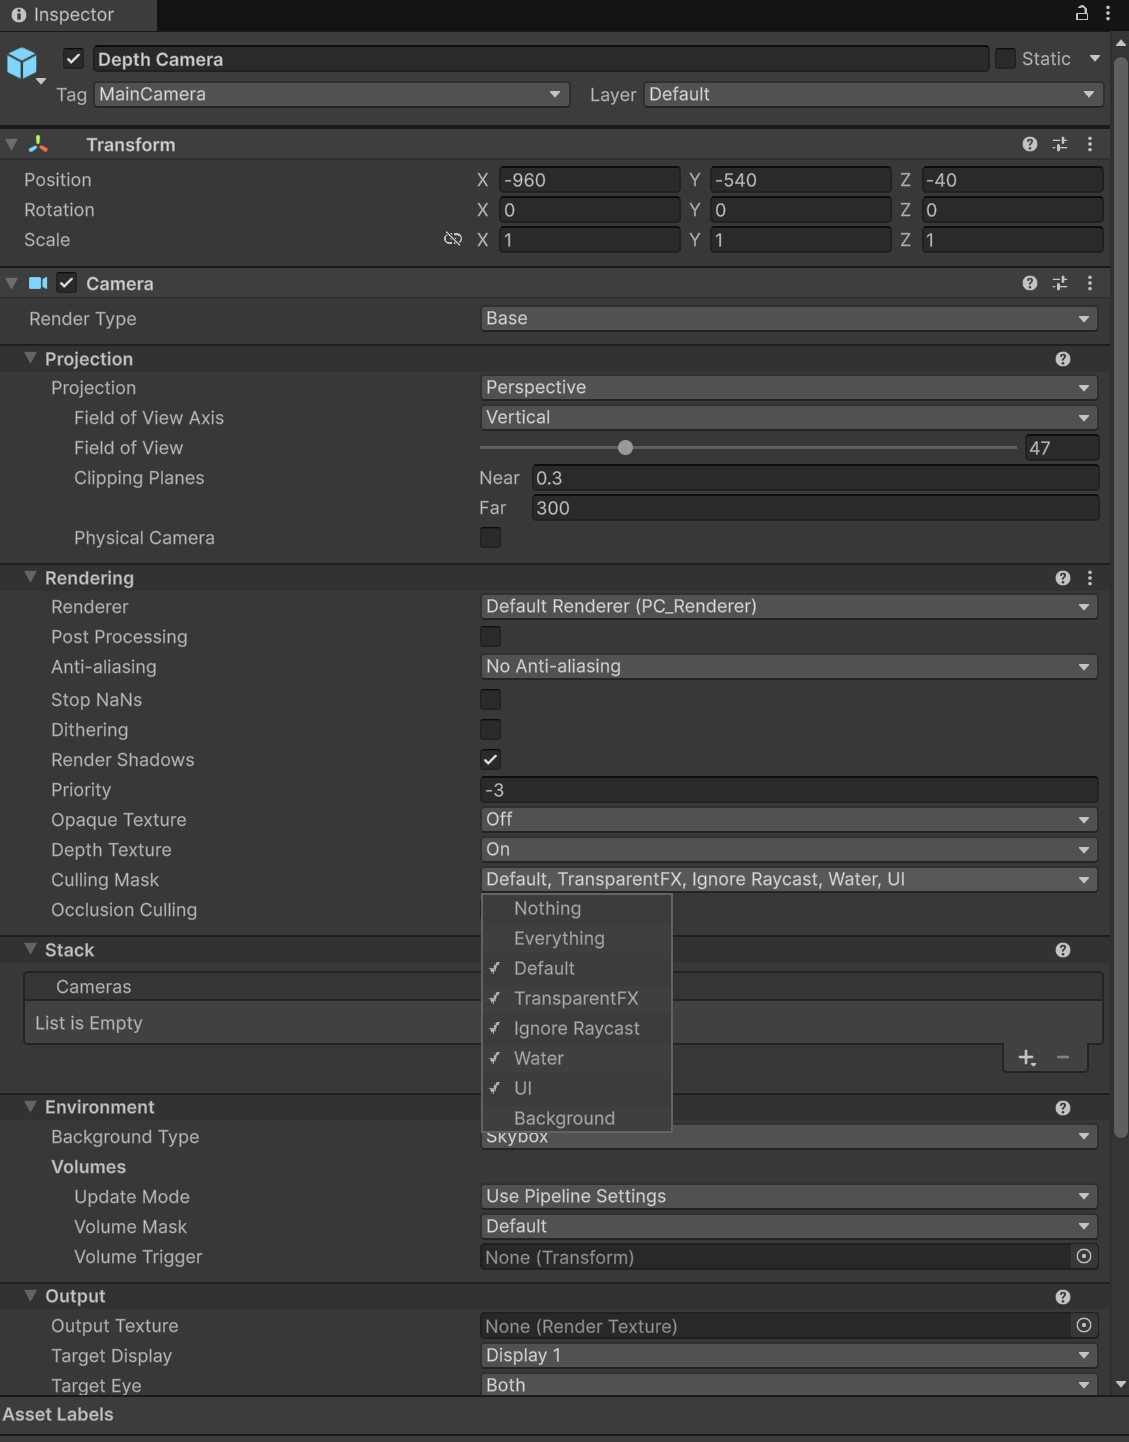
\includegraphics[width=0.7\linewidth]{images/depth_camera.png}
    \caption{Configuration du culling mask de la camera secondaire}
    \label{fig:depth_camera}
\end{figure}
Le GameObject \texttt{Depth Analysis Manager} est celui qui assure la gestion du système d'analyse de profondeur. Le compute shader associé est situé dans \texttt{assets/Resources/Shaders} nommé \texttt{Zbuffer}.
\begin{figure}[H]
    \centering
    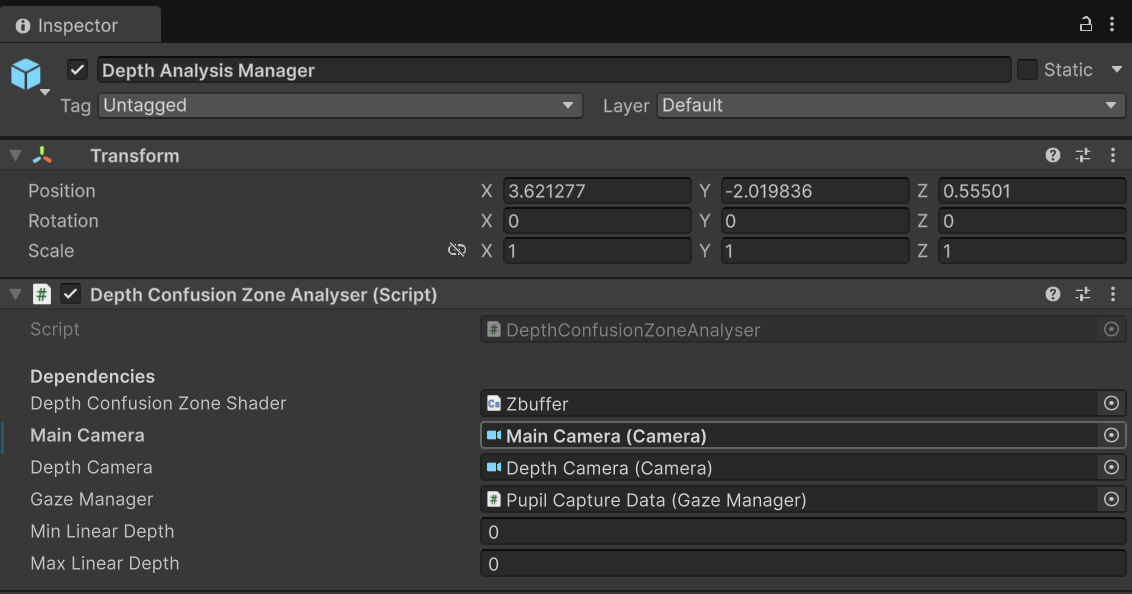
\includegraphics[width=0.5\linewidth]{images/depth_analysis_manager.png}
    \caption{Configuration de \texttt{Depth Analysis Manager}}
    \label{fig:depth_analysis_manager}
\end{figure}

\bibliography{references}
\end{document}
